\documentclass[../labs.tex]{subfiles}

\pagestyle{main}
\renewcommand{\leftmark}{Lab Report \thesection}

\begin{document}




\noindent Steven Labalme\\
26 January 2023\hfill
2 February 2023

\section{TITLE}
% \subsection{The Background Spectrum}
\begin{figure}[H]
    \centering
    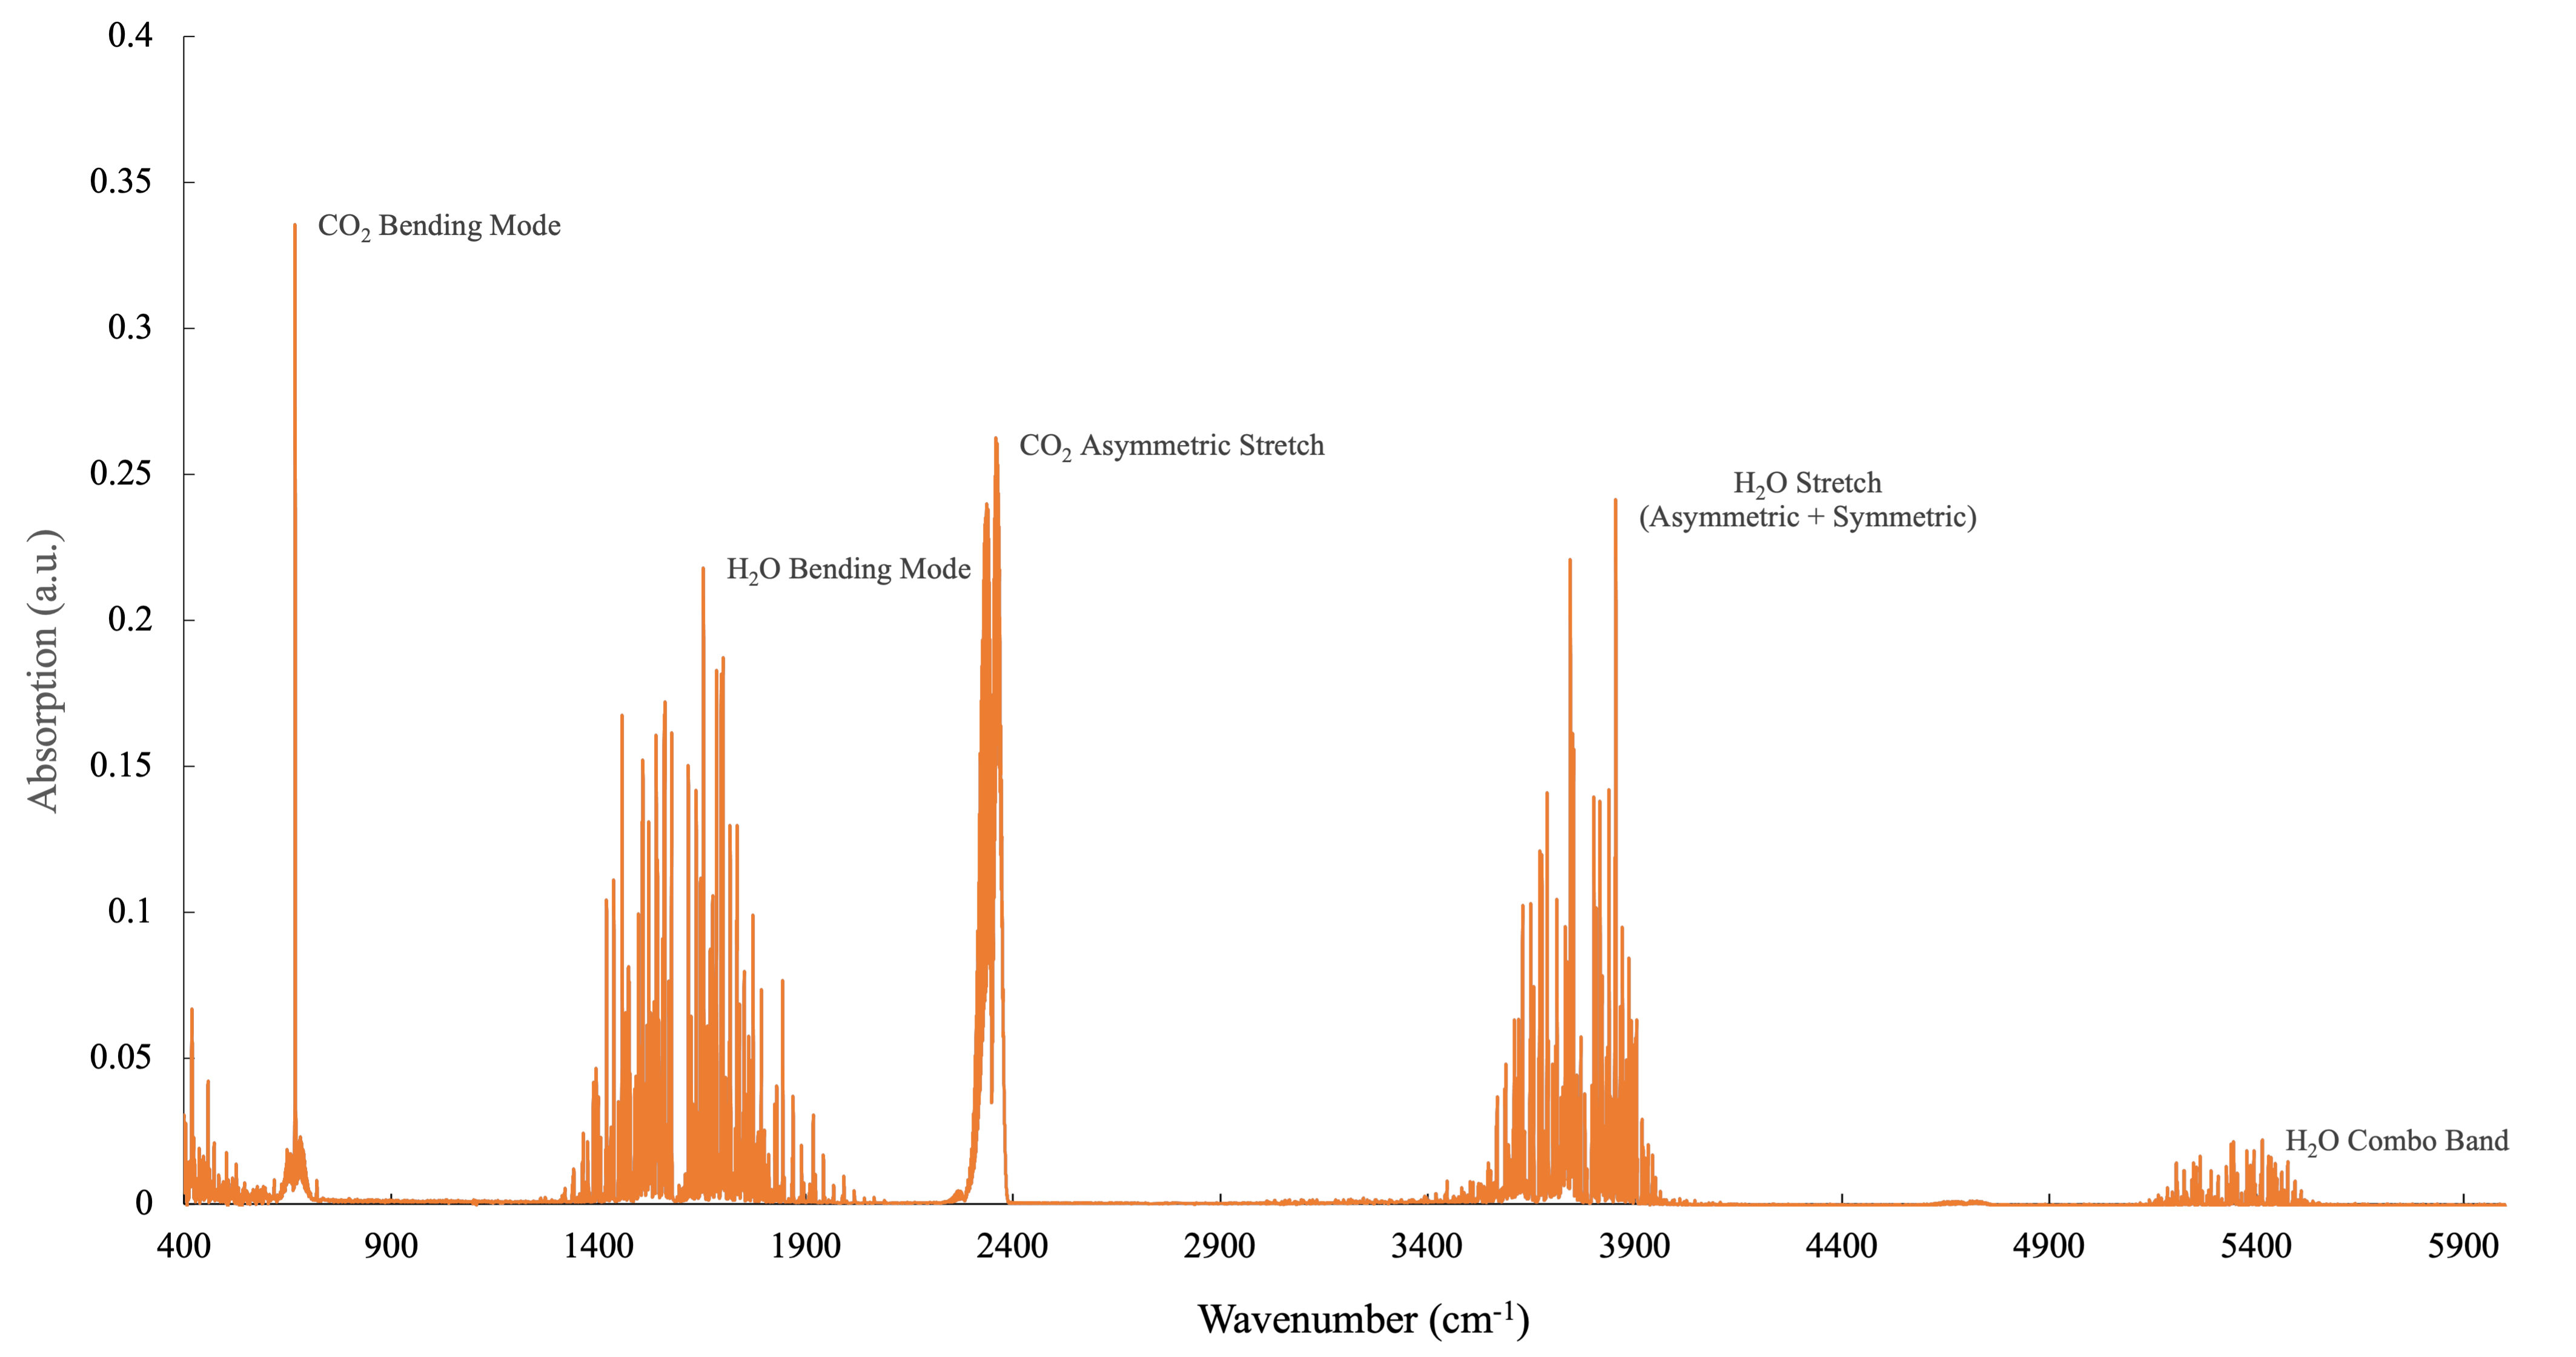
\includegraphics[width=0.98\linewidth]{lab2-background.png}
    \caption{Infrared absorption spectrum of air (background spectrum).}
    \label{fig:background}
\end{figure}

\begin{figure}[H]
    \centering
    \begin{subfigure}[b]{0.32\linewidth}
        \centering
        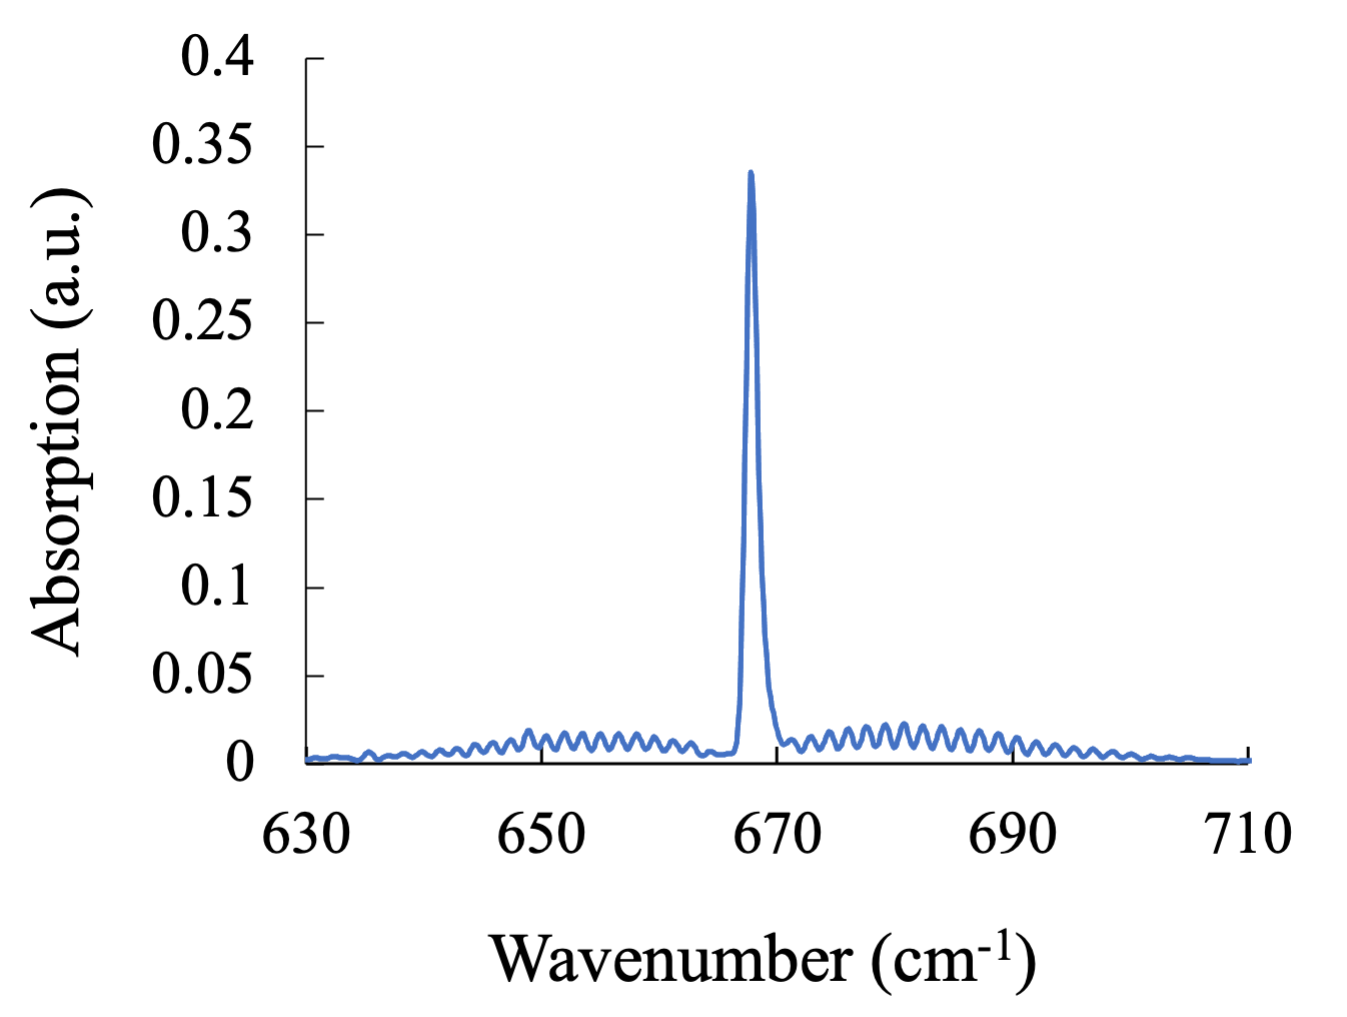
\includegraphics[width=0.9\linewidth]{lab2-peaka.png}
        \caption{\ce{CO2} bending mode.}
        \label{fig:peaka}
    \end{subfigure}
    \begin{subfigure}[b]{0.32\linewidth}
        \centering
        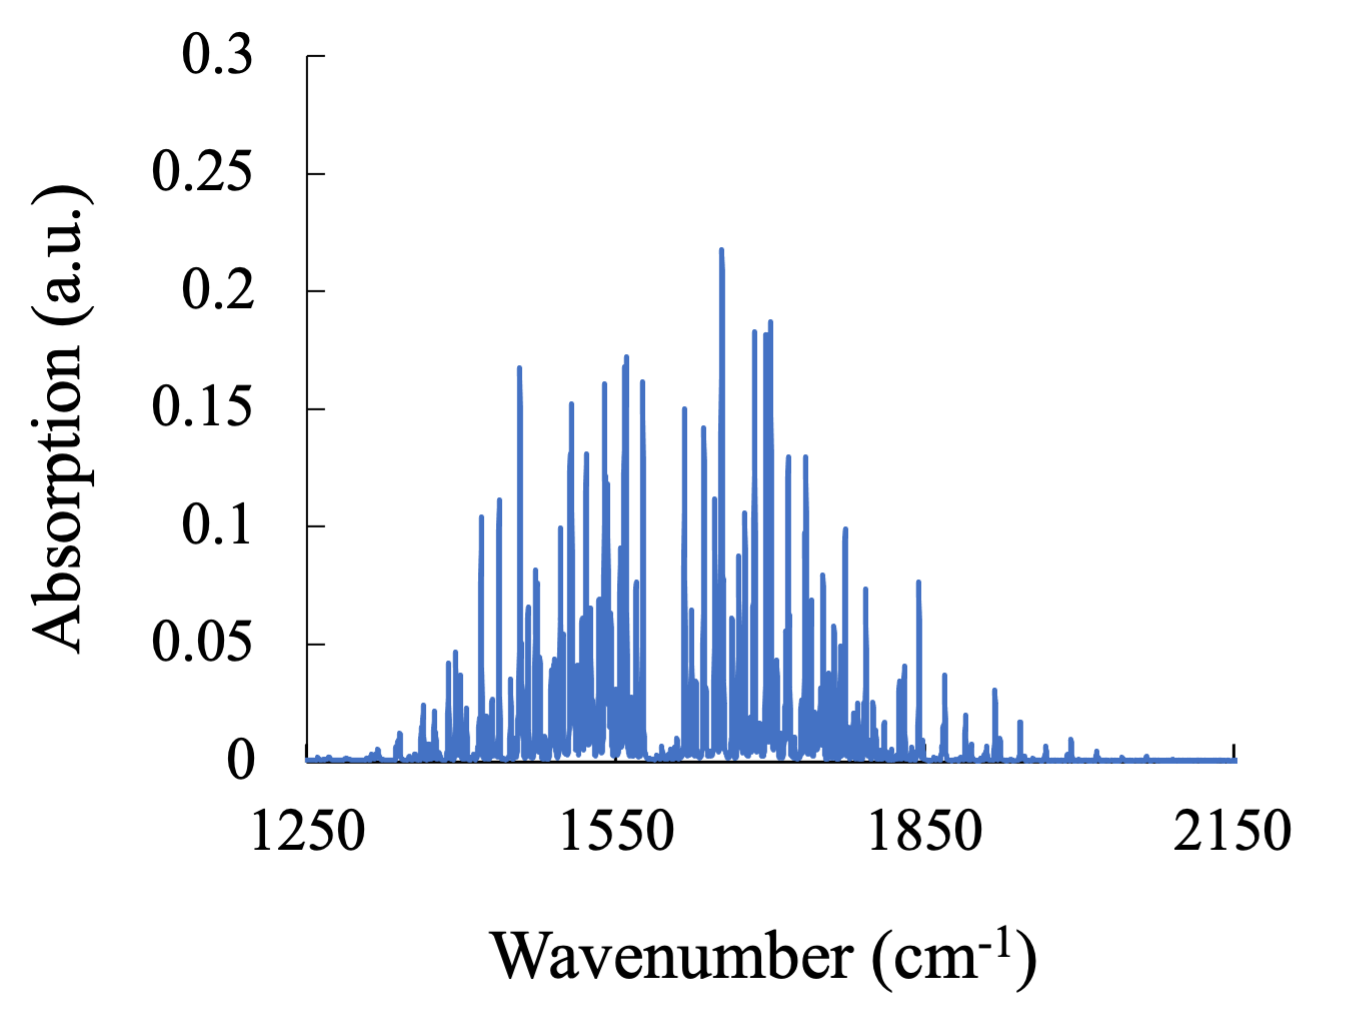
\includegraphics[width=0.9\linewidth]{lab2-peakb.png}
        \caption{\ce{H2O} bending mode.}
        \label{fig:peakb}
    \end{subfigure}
    \begin{subfigure}[b]{0.32\linewidth}
        \centering
        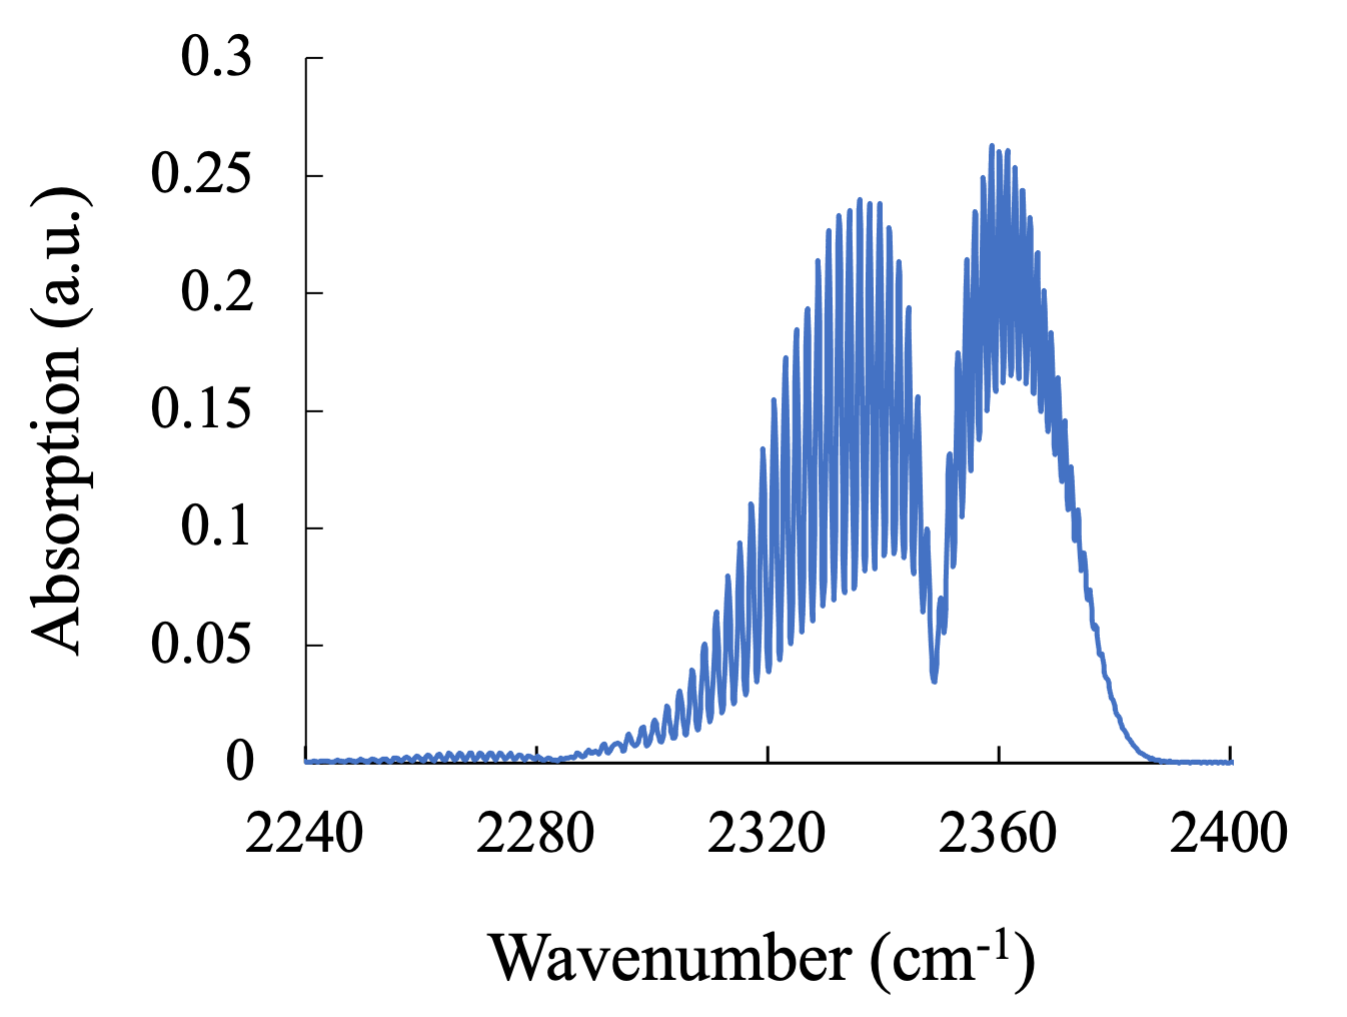
\includegraphics[width=0.9\linewidth]{lab2-peakc.png}
        \caption{\ce{CO2} asymmetric stretch.}
        \label{fig:peakc}
    \end{subfigure}\\[1em]
    \begin{subfigure}[b]{0.32\linewidth}
        \centering
        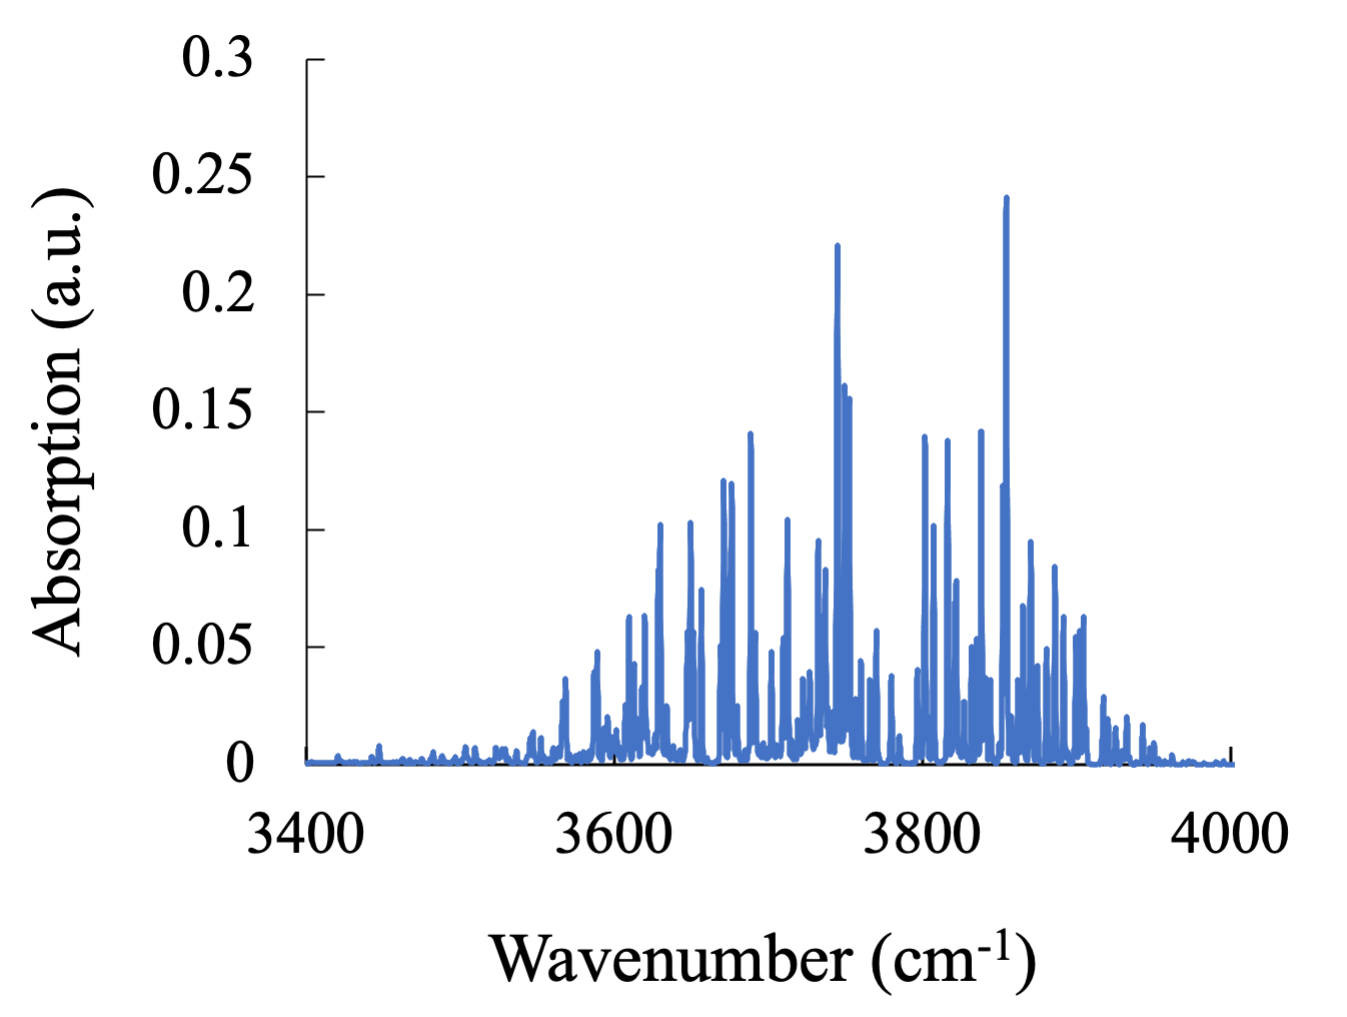
\includegraphics[width=0.9\linewidth]{lab2-peakd.png}
        \caption{\ce{H2O} stretches.}
        \label{fig:peakd}
    \end{subfigure}
    \begin{subfigure}[b]{0.32\linewidth}
        \centering
        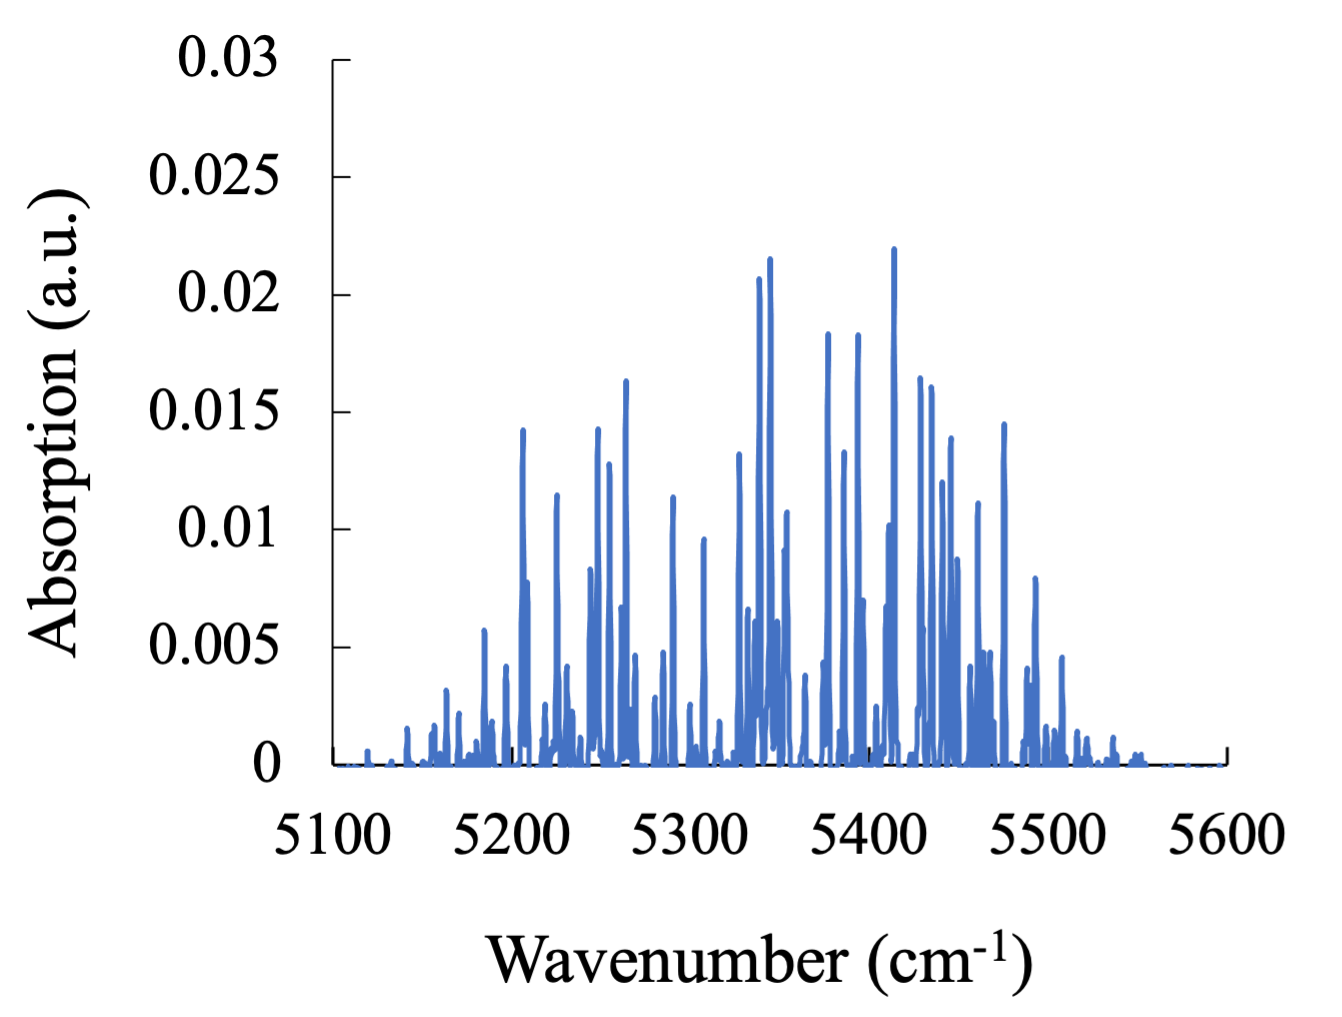
\includegraphics[width=0.9\linewidth]{lab2-peake.png}
        \caption{\ce{H2O} combo band.}
        \label{fig:peake}
    \end{subfigure}
    \caption{The five primary vibrational bands in a sample of air.}
    \label{fig:peak}
\end{figure}

\begin{table}[H]
    \centering
    \small
    \renewcommand{\arraystretch}{1.2}
    \begin{tabular}{|c|c|c|}
        \hline
        \textbf{Wavenumber Range (cm${}^{\bm{-1}}$)} & \textbf{Molecule} & \textbf{Vibrational Band}\\
        \hline
        \numrange{630}{710} & \ce{CO2} & Bending\\ \hline
        \numrange{1250}{2150} & \ce{H2O} & Bending\\ \hline
        \numrange{2240}{2400} & \ce{CO2} & Asymmetric stretch\\ \hline
        \numrange{3400}{4000} & \ce{H2O} & Asymmetric \& symmetric stretch\\ \hline
        \numrange{5100}{5600} & \ce{H2O} & Combo band\\
        \hline
    \end{tabular}
    \caption{Infrared-active vibrational modes in air molecules.}
    \label{tab:IRmodes}
\end{table}


% \subsection*{HCl}
\begin{figure}[H]
    \centering
    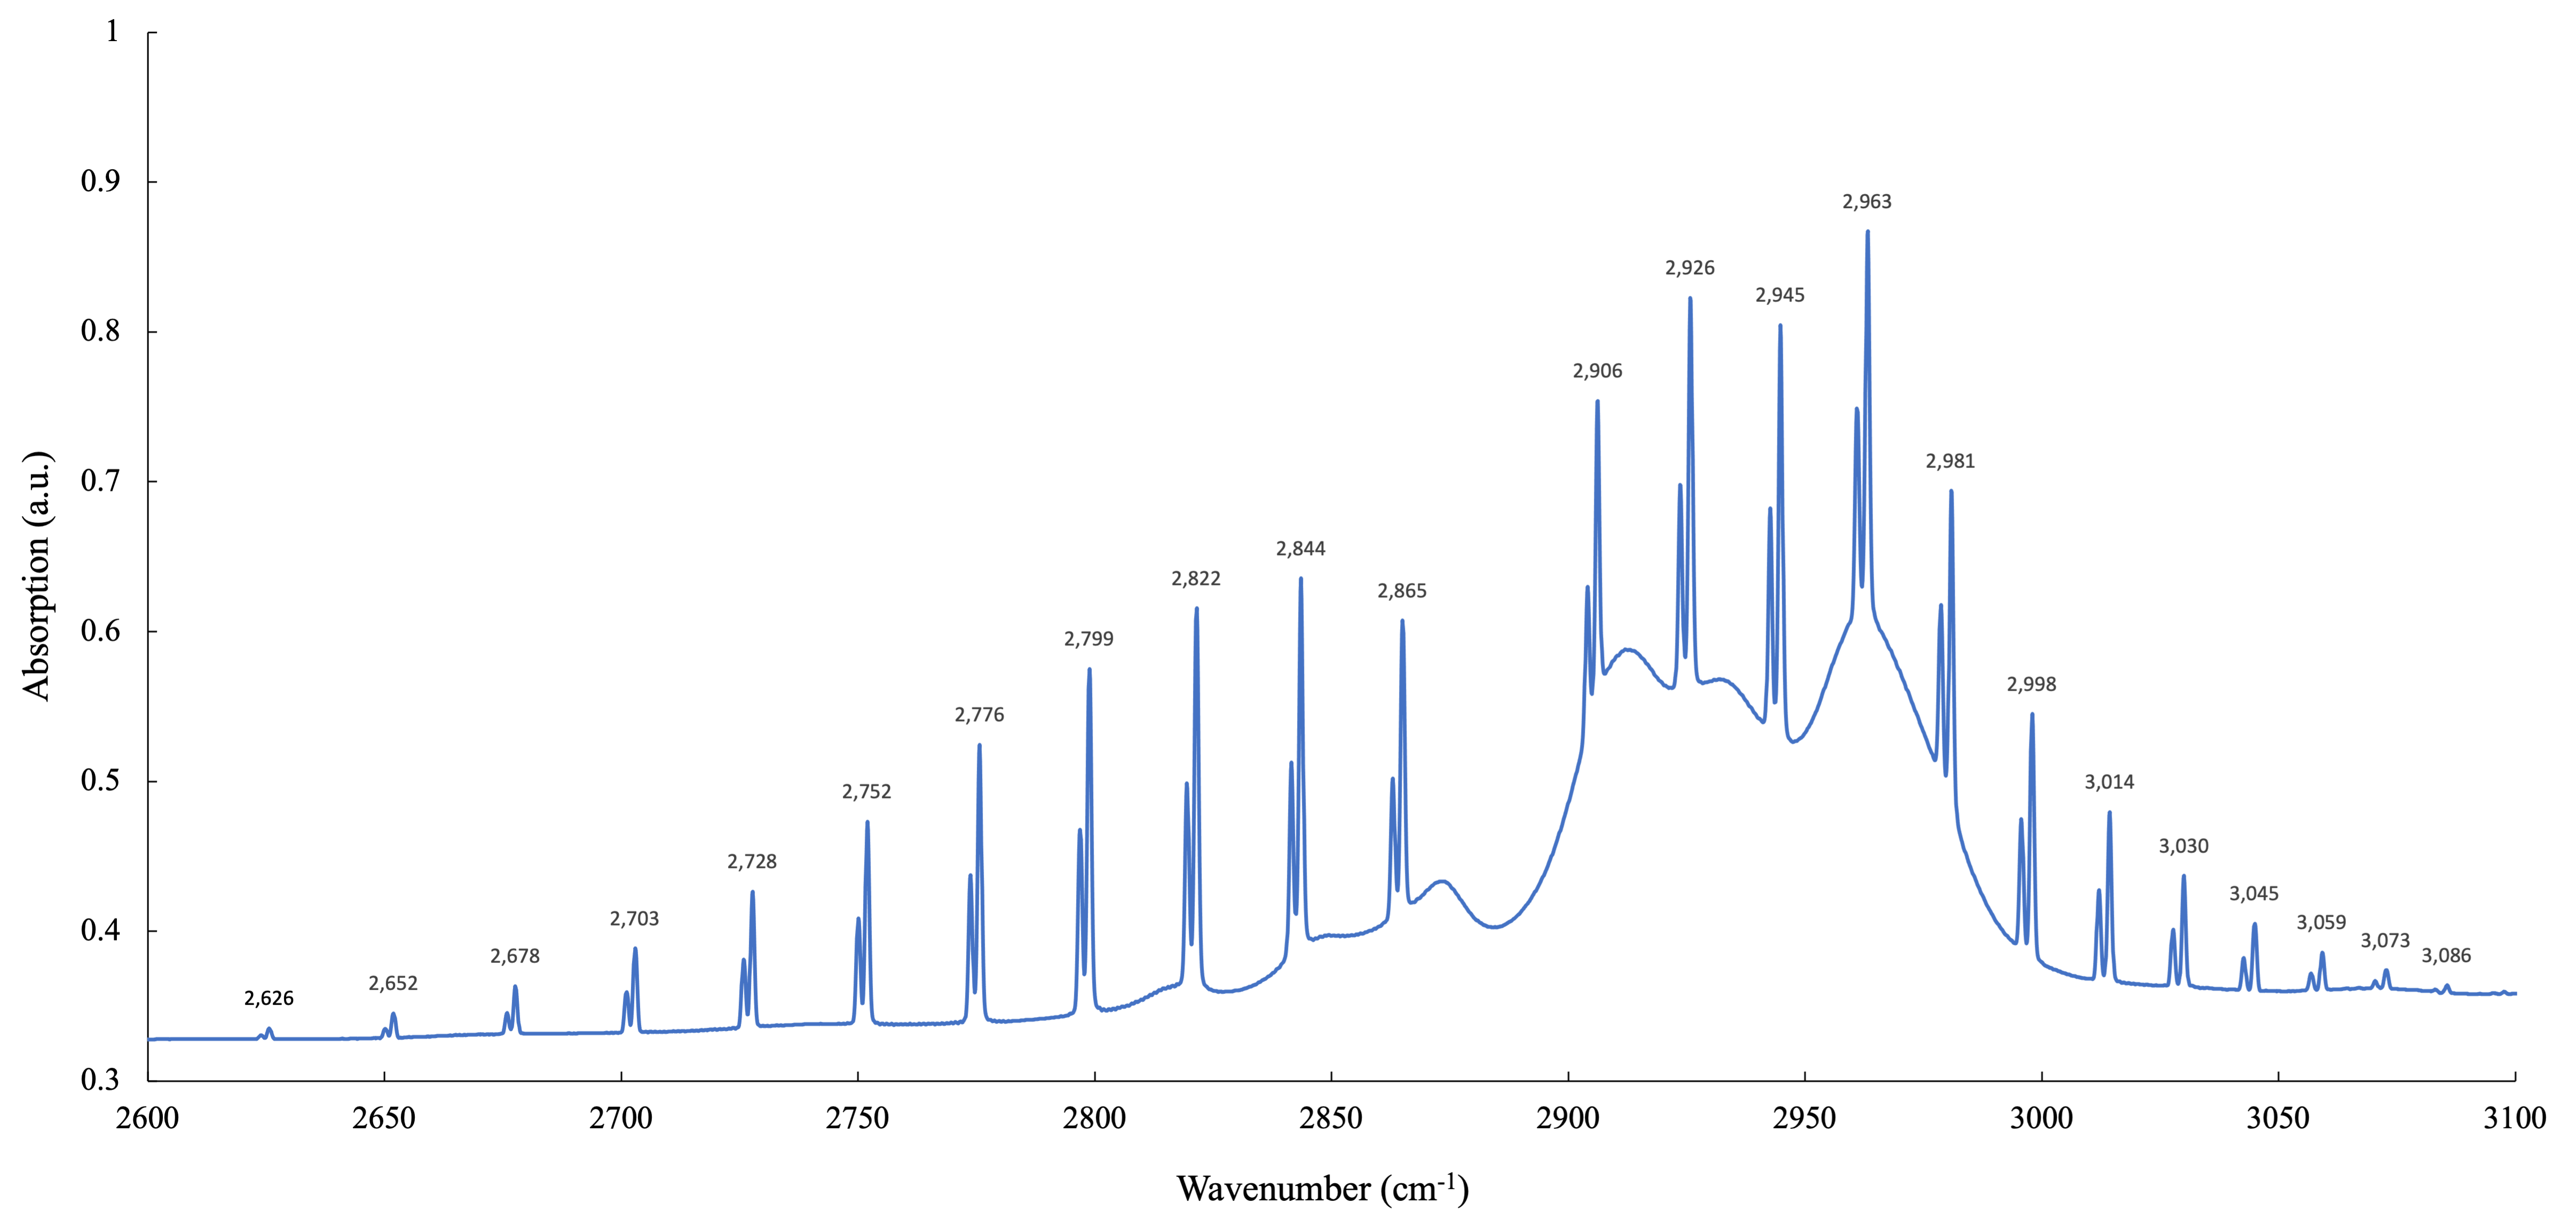
\includegraphics[width=0.98\linewidth]{lab2-rovibrationalHCl.png}
    \caption{Rovibrational absorption spectrum of \ce{HCl}.}
    \label{fig:rovibrationalHCl}
\end{figure}

\begin{figure}[H]
    \centering
    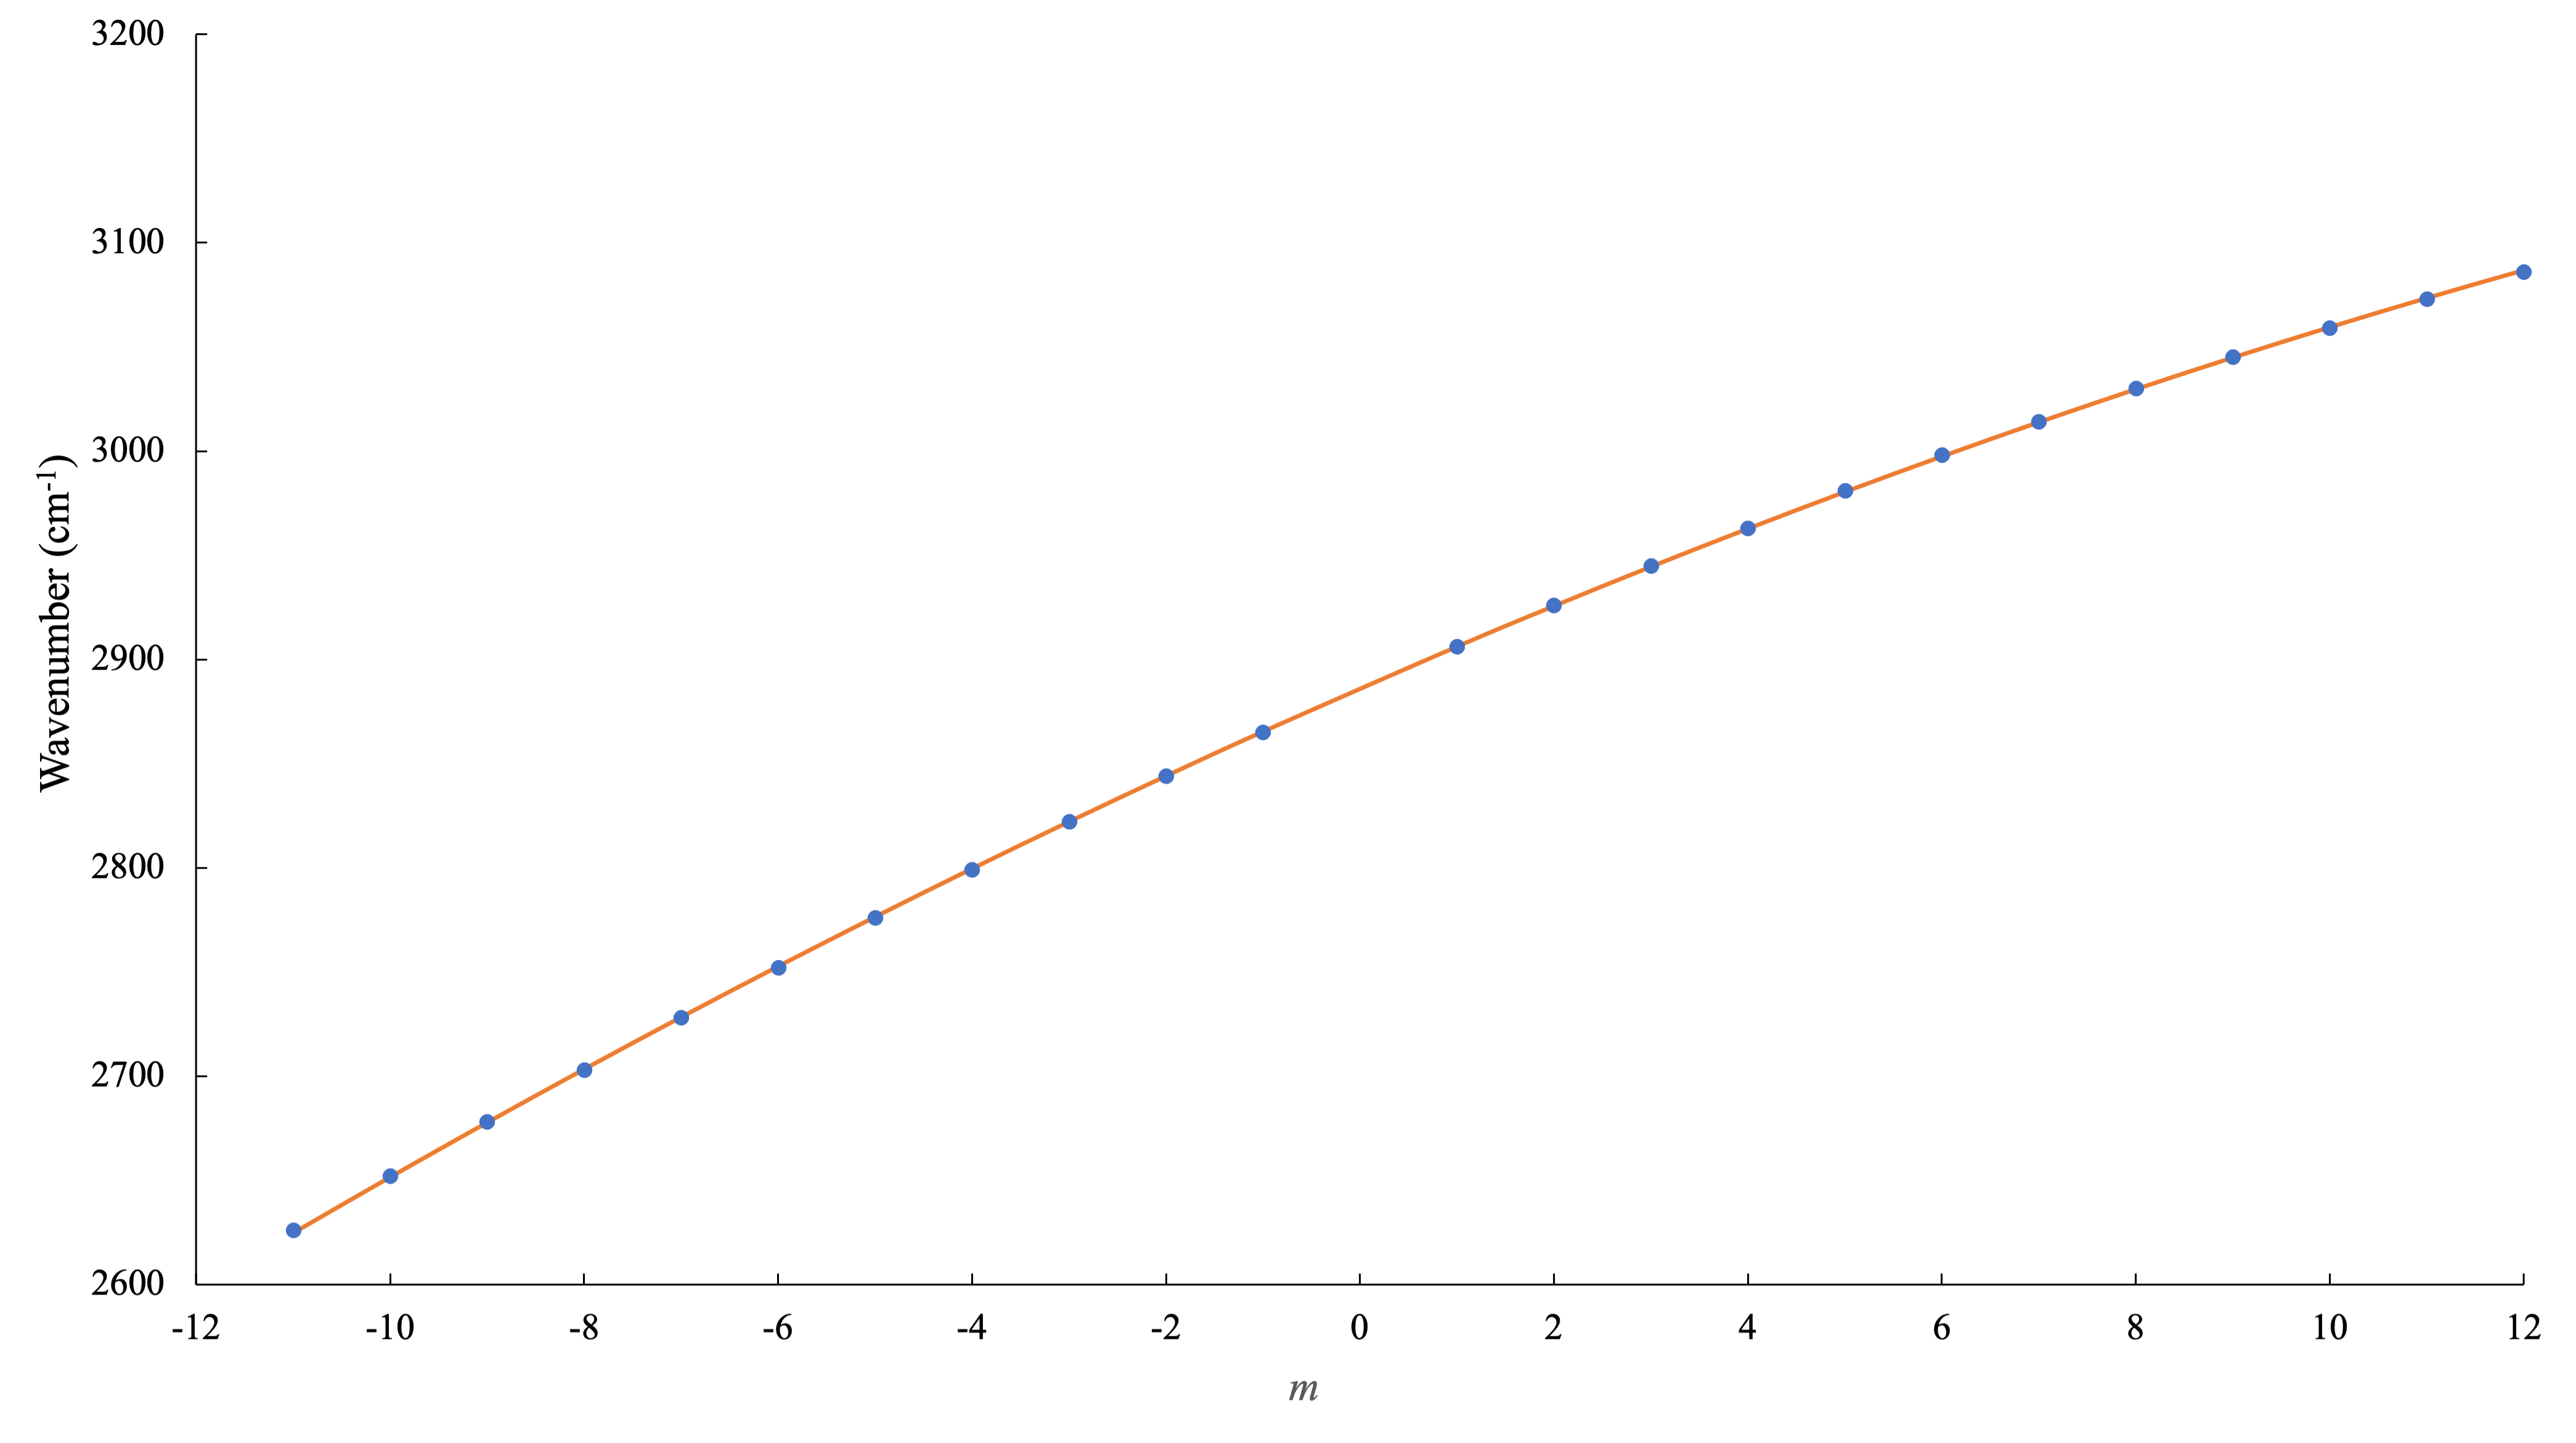
\includegraphics[width=0.98\linewidth]{lab2-vm.png}
    \begin{tikzpicture}[remember picture,overlay]
        \footnotesize
        \node at (-11,8) {$\boxed{\bar{\nu}(m)=2886+20.39m-0.3053m^2}$};
        \node at (-11,7) {$\boxed{R^2=0.998}$};
    \end{tikzpicture}
    \caption{Fitting data on the rovibrational transition wavenumbers $\bar{\nu}$ of \ce{HCl} vs. a parameter $m$ related to the rotational energy level from which such a rovibrational transition begins.}
    \label{fig:vm}
\end{figure}

\begin{table}[H]
    \centering
    \small
    \renewcommand{\arraystretch}{1.2}
    \begin{tabular}{|c|c|c|c|}
        \hline
         & $\bm{B_e}$ \textbf{(cm${}^{\bm{-1}}$)} & $\bm{\alpha_e}$ \textbf{(cm${}^{\bm{-1}}$)} & $\bm{\bar{\nu}_0}$ \textbf{(cm${}^{\bm{-1}}$)}\\ %& $\bm{I}$ \textbf{(kg\,m${}^{\bm{2}}$)} & $\bm{r_e}$ \textbf{(\AA)}\\
        \hline
        \textbf{Calculated values} & \num{10.50} & \num{0.3053} & \num{2886}\\ %& \num{2.666e-47} & \num{1.281}\\
        \hline
        \textbf{Literature values} & \num{10.59}\supercite{bib:NISTDiatomics} & \num{0.3072}\supercite{bib:NISTDiatomics} & \num{2991}\supercite{bib:NISTDiatomics}\\ %& \num{2.634e-47} & \num{1.275}\supercite{bib:NISTDiatomics}\\
        \hline
    \end{tabular}
    \caption{Calculated spectroscopic constants and their reported values.}
    \label{tab:IRConstants}
\end{table}
% Note that the "literature" value for the moment of inertia of \ce{HCl} was calculated from the equilibrium bond length in the literature via $I=\mu r_e^2$, $\mu=\SI{1.624e-27}{\kilo\gram}$.

\begin{figure}[H]
    \centering
    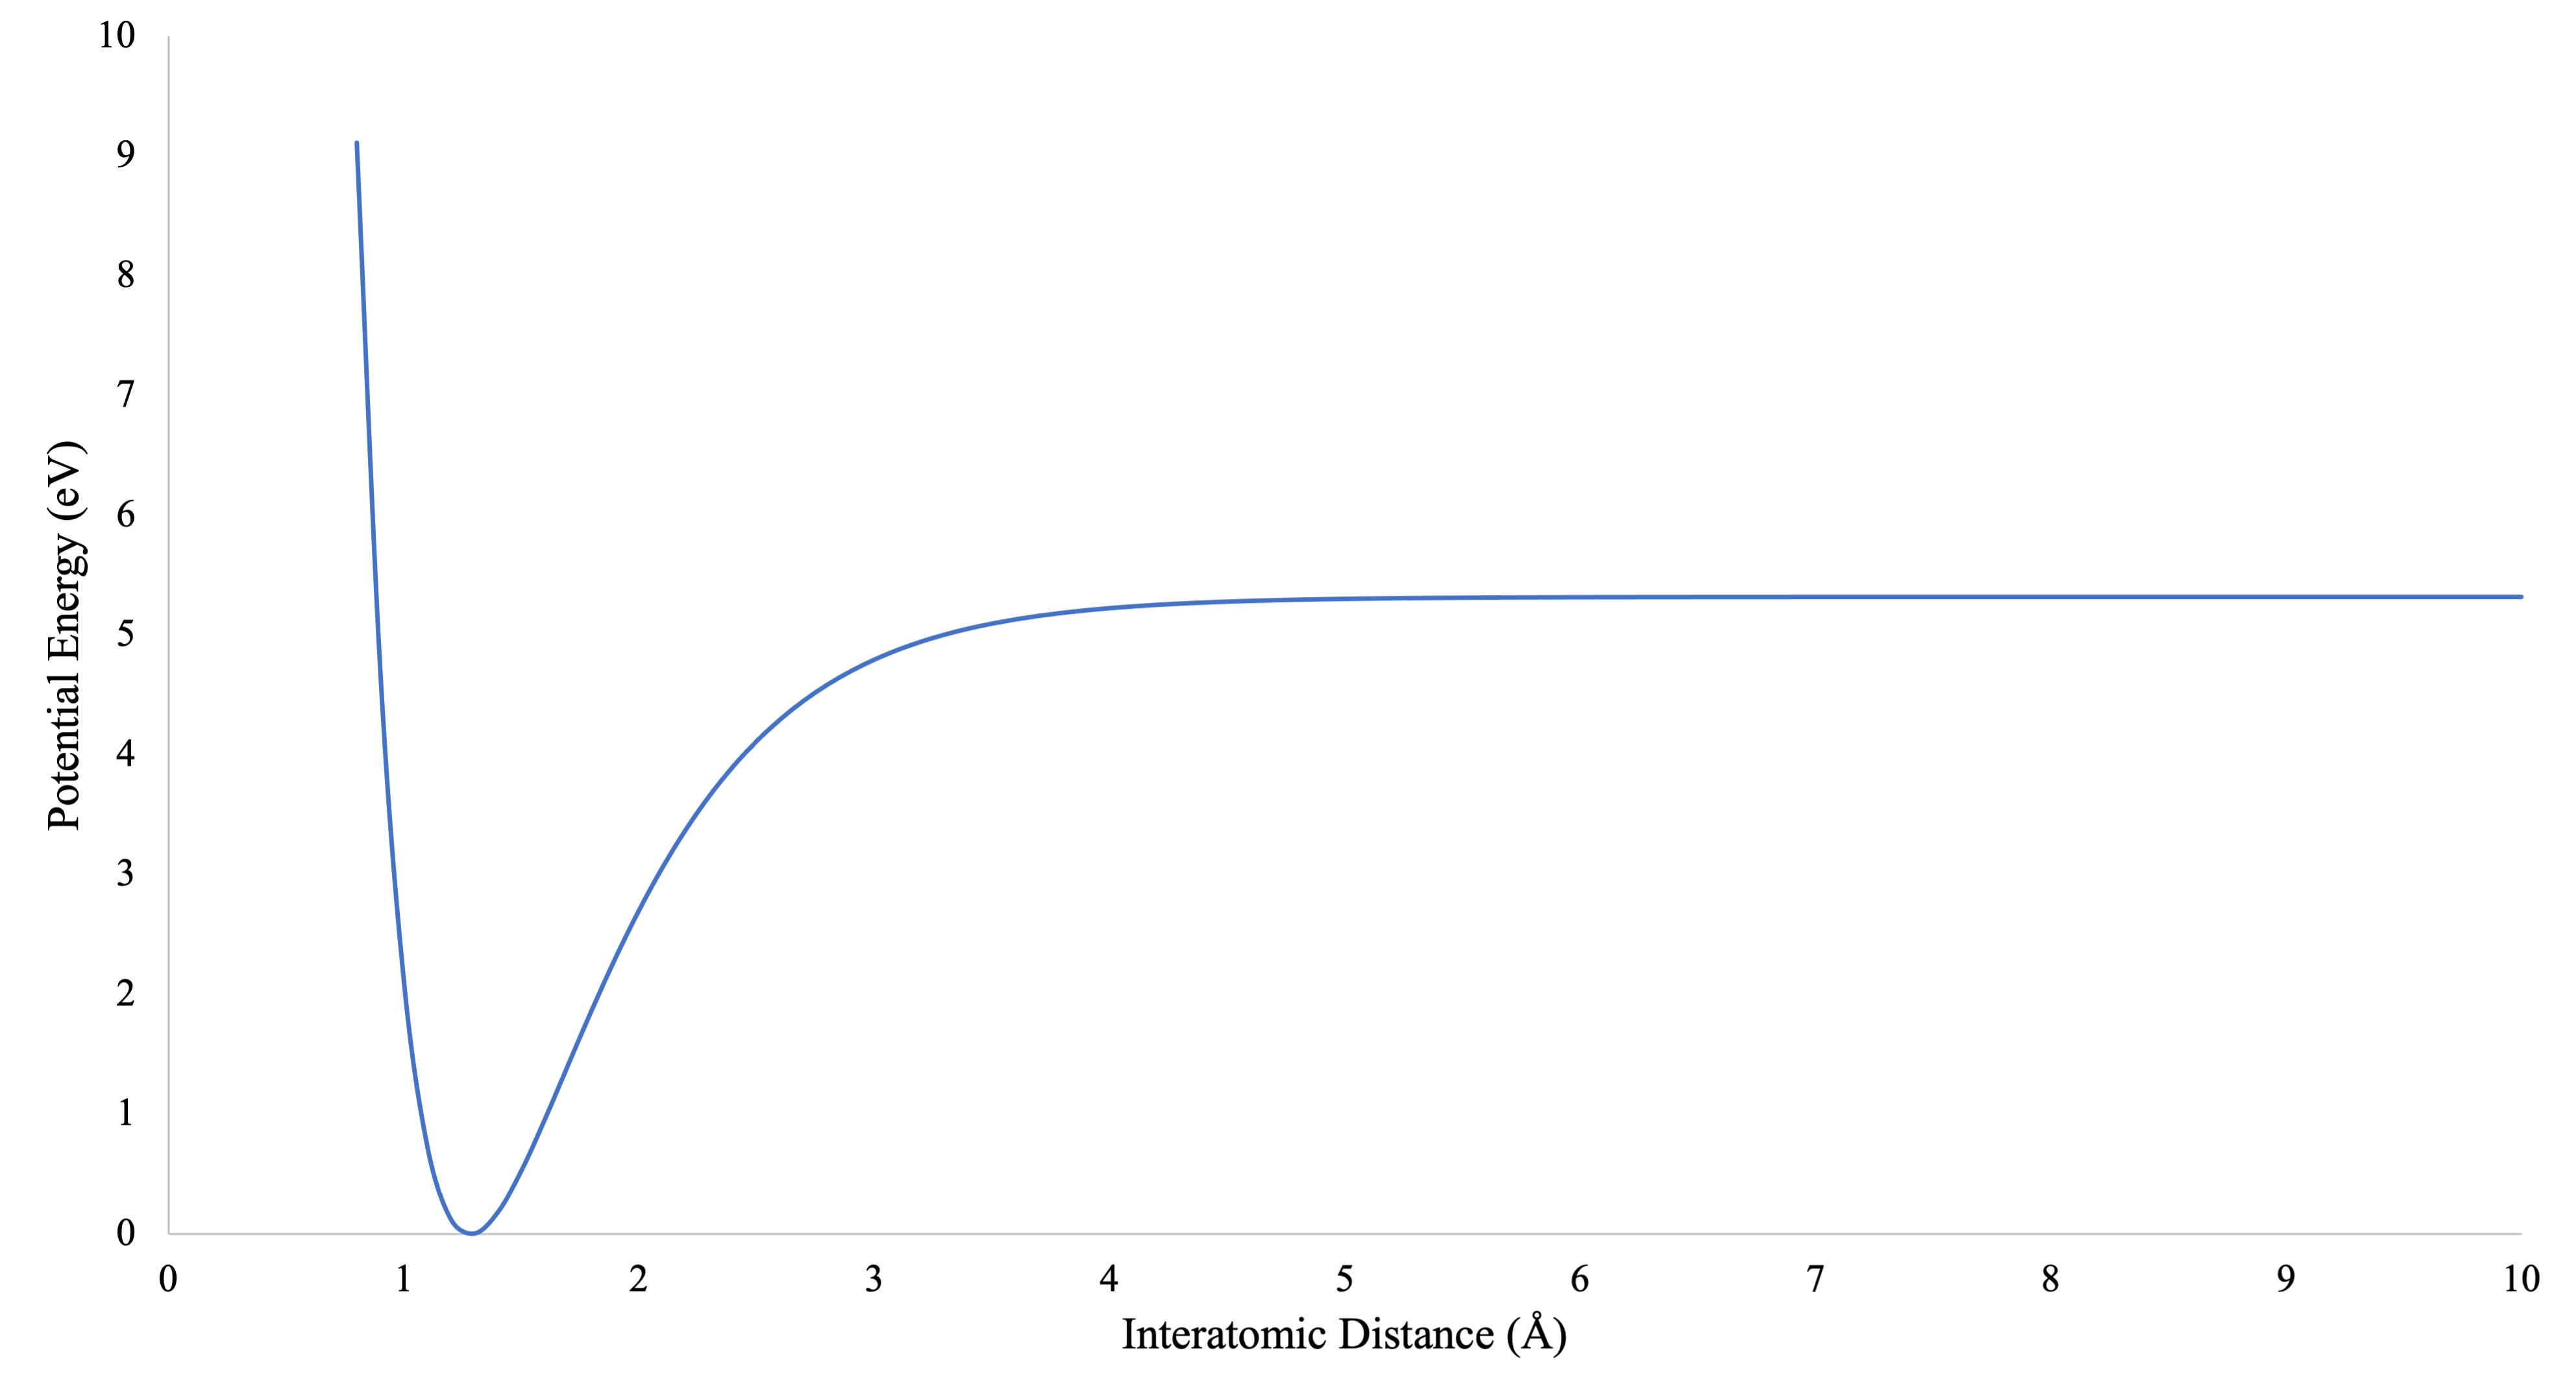
\includegraphics[width=0.98\linewidth]{lab2-morse.png}
    \caption{Morse potential curve.}
    \label{fig:morse}
\end{figure}

\begin{table}[H]
    \centering
    \small
    \renewcommand{\arraystretch}{1.2}
    \begin{tabular}{|c|c|c|c|c|}
        \hline
         & $\bm{\bar{\nu}_e}$ \textbf{(cm${}^{\bm{-1}}$)} & $\bm{x_e}$ & $\bm{D_e}$ \textbf{(eV)} & $\bm{r_e}$ \textbf{(\AA)}\\
        \hline
        \textbf{Calculated values} & \num{2990} & \num{0.01741} & \num{5.320} & \num{1.281}\\
        \hline
        \textbf{Literature values} & \num{2991}\supercite{bib:NISTDiatomics} & \num{0.01766}\supercite{bib:NISTDiatomics} & \num{5.319}\supercite{bib:NISTDiatomics} & \num{1.275}\supercite{bib:NISTDiatomics}\\
        \hline
    \end{tabular}
    \caption{Calculated energy constants and their reported values.}
    \label{tab:energyConstant}
\end{table}
\newpage


\printbibliography
\setcounter{figure}{0}
\setcounter{table}{0}




\end{document}